\documentclass[tikz,border=4pt]{standalone}
% Shared visual style. All charts remain editable vector LaTeX figures.
\usepackage[T1]{fontenc}
\usepackage{lmodern,amsmath,pgfplots}
\usepgfplotslibrary{groupplots,fillbetween,colormaps}
\usetikzlibrary{calc,positioning,plotmarks,backgrounds}
\pgfplotsset{compat=1.18}
\definecolor{abmBlue}{HTML}{0072B2}
\definecolor{abmOrange}{HTML}{D55E00}
\definecolor{abmGreen}{HTML}{009E73}
\definecolor{abmGray}{HTML}{666666}
\definecolor{abmGrid}{HTML}{E5E5E5}
\definecolor{abmLight}{HTML}{F3F3F3}
\pgfplotsset{
 abm axis/.style={
  scale only axis,font=\fontsize{9}{11}\selectfont,
  label style={font=\fontsize{9}{11}\selectfont},
  tick label style={font=\fontsize{8}{10}\selectfont},
  title style={font=\fontsize{9}{11}\selectfont,align=center},
  legend style={font=\fontsize{8}{10}\selectfont,draw=none,fill=none,cells={anchor=west}},
  axis lines=left,axis line style={black!65,line width=0.45pt},
  tick style={black!60,line width=0.4pt},major tick length=2pt,
  grid=major,grid style={draw=abmGrid,line width=0.25pt},
  scaled ticks=false,unbounded coords=jump,
  every axis plot/.append style={line width=0.8pt},
  colormap/viridis,
 },
 abm line/.style={no marks,line width=0.9pt},
 abm point/.style={only marks,mark=*,mark size=1.9pt},
}

\begin{document}
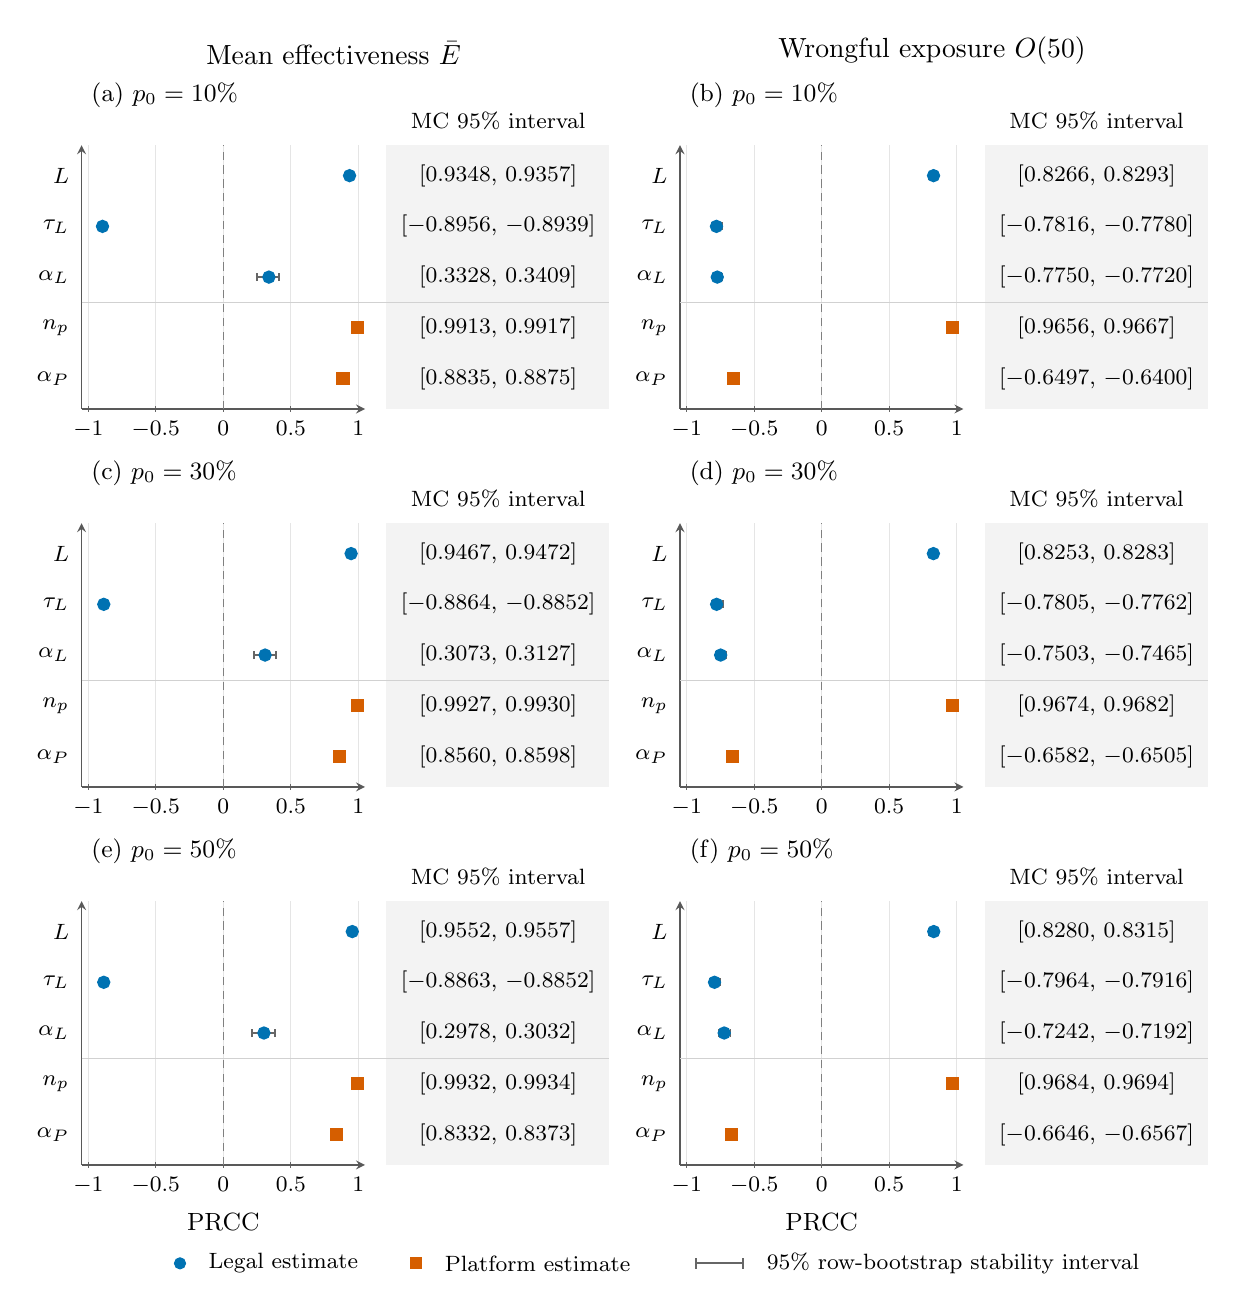
\begin{tikzpicture}

% Source: supplied data/figS2b_PRCC/source.csv, validated separately.
% derived/prcc_*.csv adds only plot_y; all statistical fields retain source strings.
\begin{groupplot}[abm axis,group style={group size=2 by 3,horizontal sep=4.0cm,vertical sep=1.45cm},
 width=3.6cm,height=3.35cm,xmin=-1.05,xmax=1.05,xtick={-1,-0.5,0,0.5,1},
 ymin=-0.6,ymax=4.6,ytick={4,3,2,1,0},yticklabels={$L$,$\tau_L$,$\alpha_L$,$n_p$,$\alpha_P$},
 xlabel={PRCC},ymajorgrids=false,ytick style={draw=none},clip=false,
 title style={at={(0,1)},anchor=south west,yshift=4pt}]

\nextgroupplot[title={(a) $p_0=10\%$},xlabel={}]
\addplot[black!50,densely dashed,line width=0.45pt,forget plot] coordinates {(0,-0.6) (0,4.6)};
\addplot[abmGray,line width=0.65pt,forget plot] coordinates {(0.917432178741,4) (0.948323751998,4)};
\draw[abmGray,line width=0.65pt] (axis cs:0.917432178741,3.92)--(axis cs:0.917432178741,4.08) (axis cs:0.948323751998,3.92)--(axis cs:0.948323751998,4.08);
\addplot[only marks,mark=*,mark size=2pt,abmBlue,forget plot] coordinates {(0.935329673664,4)};
\addplot[abmGray,line width=0.65pt,forget plot] coordinates {(-0.910364459861,3) (-0.875407520304,3)};
\draw[abmGray,line width=0.65pt] (axis cs:-0.910364459861,2.92)--(axis cs:-0.910364459861,3.08) (axis cs:-0.875407520304,2.92)--(axis cs:-0.875407520304,3.08);
\addplot[only marks,mark=*,mark size=2pt,abmBlue,forget plot] coordinates {(-0.894951809376,3)};
\addplot[abmGray,line width=0.65pt,forget plot] coordinates {(0.251309995923,2) (0.40970392019,2)};
\draw[abmGray,line width=0.65pt] (axis cs:0.251309995923,1.92)--(axis cs:0.251309995923,2.08) (axis cs:0.40970392019,1.92)--(axis cs:0.40970392019,2.08);
\addplot[only marks,mark=*,mark size=2pt,abmBlue,forget plot] coordinates {(0.337766849657,2)};
\addplot[abmGray,line width=0.65pt,forget plot] coordinates {(0.988245563629,1) (0.993133747071,1)};
\draw[abmGray,line width=0.65pt] (axis cs:0.988245563629,0.92)--(axis cs:0.988245563629,1.08) (axis cs:0.993133747071,0.92)--(axis cs:0.993133747071,1.08);
\addplot[only marks,mark=square*,mark size=2pt,abmOrange,forget plot] coordinates {(0.991638720604,1)};
\addplot[abmGray,line width=0.65pt,forget plot] coordinates {(0.853808666108,0) (0.900918847882,0)};
\draw[abmGray,line width=0.65pt] (axis cs:0.853808666108,-0.08)--(axis cs:0.853808666108,0.08) (axis cs:0.900918847882,-0.08)--(axis cs:0.900918847882,0.08);
\addplot[only marks,mark=square*,mark size=2pt,abmOrange,forget plot] coordinates {(0.887001616984,0)};
\fill[abmLight] ([xshift=0.27cm]rel axis cs:1,0) rectangle ([xshift=3.10cm]rel axis cs:1,1);
\node[anchor=south,font=\fontsize{8}{10}\selectfont] at ([xshift=1.69cm,yshift=2pt]rel axis cs:1,1) {MC 95\% interval};
\draw[black!18,line width=0.35pt] (rel axis cs:0,0.40385)--([xshift=3.10cm]rel axis cs:1,0.40385);

\node[font=\fontsize{8}{10}\selectfont,anchor=center] at ([xshift=1.69cm]axis cs:1.05,4) {$[0.9348,\,0.9357]$};
\node[font=\fontsize{8}{10}\selectfont,anchor=center] at ([xshift=1.69cm]axis cs:1.05,3) {$[-0.8956,\,-0.8939]$};
\node[font=\fontsize{8}{10}\selectfont,anchor=center] at ([xshift=1.69cm]axis cs:1.05,2) {$[0.3328,\,0.3409]$};
\node[font=\fontsize{8}{10}\selectfont,anchor=center] at ([xshift=1.69cm]axis cs:1.05,1) {$[0.9913,\,0.9917]$};
\node[font=\fontsize{8}{10}\selectfont,anchor=center] at ([xshift=1.69cm]axis cs:1.05,0) {$[0.8835,\,0.8875]$};
\nextgroupplot[title={(b) $p_0=10\%$},xlabel={}]
\addplot[black!50,densely dashed,line width=0.45pt,forget plot] coordinates {(0,-0.6) (0,4.6)};
\addplot[abmGray,line width=0.65pt,forget plot] coordinates {(0.794255681308,4) (0.856720363753,4)};
\draw[abmGray,line width=0.65pt] (axis cs:0.794255681308,3.92)--(axis cs:0.794255681308,4.08) (axis cs:0.856720363753,3.92)--(axis cs:0.856720363753,4.08);
\addplot[only marks,mark=*,mark size=2pt,abmBlue,forget plot] coordinates {(0.828305602263,4)};
\addplot[abmGray,line width=0.65pt,forget plot] coordinates {(-0.816134251333,3) (-0.740323962234,3)};
\draw[abmGray,line width=0.65pt] (axis cs:-0.816134251333,2.92)--(axis cs:-0.816134251333,3.08) (axis cs:-0.740323962234,2.92)--(axis cs:-0.740323962234,3.08);
\addplot[only marks,mark=*,mark size=2pt,abmBlue,forget plot] coordinates {(-0.779984788655,3)};
\addplot[abmGray,line width=0.65pt,forget plot] coordinates {(-0.806846119196,2) (-0.734703442298,2)};
\draw[abmGray,line width=0.65pt] (axis cs:-0.806846119196,1.92)--(axis cs:-0.806846119196,2.08) (axis cs:-0.734703442298,1.92)--(axis cs:-0.734703442298,2.08);
\addplot[only marks,mark=*,mark size=2pt,abmBlue,forget plot] coordinates {(-0.77386662872,2)};
\addplot[abmGray,line width=0.65pt,forget plot] coordinates {(0.956069165994,1) (0.974964681636,1)};
\draw[abmGray,line width=0.65pt] (axis cs:0.956069165994,0.92)--(axis cs:0.956069165994,1.08) (axis cs:0.974964681636,0.92)--(axis cs:0.974964681636,1.08);
\addplot[only marks,mark=square*,mark size=2pt,abmOrange,forget plot] coordinates {(0.966744228203,1)};
\addplot[abmGray,line width=0.65pt,forget plot] coordinates {(-0.686926056552,0) (-0.611271019394,0)};
\draw[abmGray,line width=0.65pt] (axis cs:-0.686926056552,-0.08)--(axis cs:-0.686926056552,0.08) (axis cs:-0.611271019394,-0.08)--(axis cs:-0.611271019394,0.08);
\addplot[only marks,mark=square*,mark size=2pt,abmOrange,forget plot] coordinates {(-0.651287694874,0)};
\fill[abmLight] ([xshift=0.27cm]rel axis cs:1,0) rectangle ([xshift=3.10cm]rel axis cs:1,1);
\node[anchor=south,font=\fontsize{8}{10}\selectfont] at ([xshift=1.69cm,yshift=2pt]rel axis cs:1,1) {MC 95\% interval};
\draw[black!18,line width=0.35pt] (rel axis cs:0,0.40385)--([xshift=3.10cm]rel axis cs:1,0.40385);

\node[font=\fontsize{8}{10}\selectfont,anchor=center] at ([xshift=1.69cm]axis cs:1.05,4) {$[0.8266,\,0.8293]$};
\node[font=\fontsize{8}{10}\selectfont,anchor=center] at ([xshift=1.69cm]axis cs:1.05,3) {$[-0.7816,\,-0.7780]$};
\node[font=\fontsize{8}{10}\selectfont,anchor=center] at ([xshift=1.69cm]axis cs:1.05,2) {$[-0.7750,\,-0.7720]$};
\node[font=\fontsize{8}{10}\selectfont,anchor=center] at ([xshift=1.69cm]axis cs:1.05,1) {$[0.9656,\,0.9667]$};
\node[font=\fontsize{8}{10}\selectfont,anchor=center] at ([xshift=1.69cm]axis cs:1.05,0) {$[-0.6497,\,-0.6400]$};
\nextgroupplot[title={(c) $p_0=30\%$},xlabel={}]
\addplot[black!50,densely dashed,line width=0.45pt,forget plot] coordinates {(0,-0.6) (0,4.6)};
\addplot[abmGray,line width=0.65pt,forget plot] coordinates {(0.932401004519,4) (0.955872966841,4)};
\draw[abmGray,line width=0.65pt] (axis cs:0.932401004519,3.92)--(axis cs:0.932401004519,4.08) (axis cs:0.955872966841,3.92)--(axis cs:0.955872966841,4.08);
\addplot[only marks,mark=*,mark size=2pt,abmBlue,forget plot] coordinates {(0.946796938876,4)};
\addplot[abmGray,line width=0.65pt,forget plot] coordinates {(-0.900531627021,3) (-0.86306283894,3)};
\draw[abmGray,line width=0.65pt] (axis cs:-0.900531627021,2.92)--(axis cs:-0.900531627021,3.08) (axis cs:-0.86306283894,2.92)--(axis cs:-0.86306283894,3.08);
\addplot[only marks,mark=*,mark size=2pt,abmBlue,forget plot] coordinates {(-0.885557773504,3)};
\addplot[abmGray,line width=0.65pt,forget plot] coordinates {(0.22983427805,2) (0.38889937195,2)};
\draw[abmGray,line width=0.65pt] (axis cs:0.22983427805,1.92)--(axis cs:0.22983427805,2.08) (axis cs:0.38889937195,1.92)--(axis cs:0.38889937195,2.08);
\addplot[only marks,mark=*,mark size=2pt,abmBlue,forget plot] coordinates {(0.309610409799,2)};
\addplot[abmGray,line width=0.65pt,forget plot] coordinates {(0.989505379869,1) (0.994369099999,1)};
\draw[abmGray,line width=0.65pt] (axis cs:0.989505379869,0.92)--(axis cs:0.989505379869,1.08) (axis cs:0.994369099999,0.92)--(axis cs:0.994369099999,1.08);
\addplot[only marks,mark=square*,mark size=2pt,abmOrange,forget plot] coordinates {(0.992871252095,1)};
\addplot[abmGray,line width=0.65pt,forget plot] coordinates {(0.817983658478,0) (0.875857607758,0)};
\draw[abmGray,line width=0.65pt] (axis cs:0.817983658478,-0.08)--(axis cs:0.817983658478,0.08) (axis cs:0.875857607758,-0.08)--(axis cs:0.875857607758,0.08);
\addplot[only marks,mark=square*,mark size=2pt,abmOrange,forget plot] coordinates {(0.858508922056,0)};
\fill[abmLight] ([xshift=0.27cm]rel axis cs:1,0) rectangle ([xshift=3.10cm]rel axis cs:1,1);
\node[anchor=south,font=\fontsize{8}{10}\selectfont] at ([xshift=1.69cm,yshift=2pt]rel axis cs:1,1) {MC 95\% interval};
\draw[black!18,line width=0.35pt] (rel axis cs:0,0.40385)--([xshift=3.10cm]rel axis cs:1,0.40385);

\node[font=\fontsize{8}{10}\selectfont,anchor=center] at ([xshift=1.69cm]axis cs:1.05,4) {$[0.9467,\,0.9472]$};
\node[font=\fontsize{8}{10}\selectfont,anchor=center] at ([xshift=1.69cm]axis cs:1.05,3) {$[-0.8864,\,-0.8852]$};
\node[font=\fontsize{8}{10}\selectfont,anchor=center] at ([xshift=1.69cm]axis cs:1.05,2) {$[0.3073,\,0.3127]$};
\node[font=\fontsize{8}{10}\selectfont,anchor=center] at ([xshift=1.69cm]axis cs:1.05,1) {$[0.9927,\,0.9930]$};
\node[font=\fontsize{8}{10}\selectfont,anchor=center] at ([xshift=1.69cm]axis cs:1.05,0) {$[0.8560,\,0.8598]$};
\nextgroupplot[title={(d) $p_0=30\%$},xlabel={}]
\addplot[black!50,densely dashed,line width=0.45pt,forget plot] coordinates {(0,-0.6) (0,4.6)};
\addplot[abmGray,line width=0.65pt,forget plot] coordinates {(0.792252947351,4) (0.854734617741,4)};
\draw[abmGray,line width=0.65pt] (axis cs:0.792252947351,3.92)--(axis cs:0.792252947351,4.08) (axis cs:0.854734617741,3.92)--(axis cs:0.854734617741,4.08);
\addplot[only marks,mark=*,mark size=2pt,abmBlue,forget plot] coordinates {(0.827141483865,4)};
\addplot[abmGray,line width=0.65pt,forget plot] coordinates {(-0.816499939588,3) (-0.732515317668,3)};
\draw[abmGray,line width=0.65pt] (axis cs:-0.816499939588,2.92)--(axis cs:-0.816499939588,3.08) (axis cs:-0.732515317668,2.92)--(axis cs:-0.732515317668,3.08);
\addplot[only marks,mark=*,mark size=2pt,abmBlue,forget plot] coordinates {(-0.778762414854,3)};
\addplot[abmGray,line width=0.65pt,forget plot] coordinates {(-0.783181921298,2) (-0.706734468424,2)};
\draw[abmGray,line width=0.65pt] (axis cs:-0.783181921298,1.92)--(axis cs:-0.783181921298,2.08) (axis cs:-0.706734468424,1.92)--(axis cs:-0.706734468424,2.08);
\addplot[only marks,mark=*,mark size=2pt,abmBlue,forget plot] coordinates {(-0.749155363828,2)};
\addplot[abmGray,line width=0.65pt,forget plot] coordinates {(0.958825969246,1) (0.977136894477,1)};
\draw[abmGray,line width=0.65pt] (axis cs:0.958825969246,0.92)--(axis cs:0.958825969246,1.08) (axis cs:0.977136894477,0.92)--(axis cs:0.977136894477,1.08);
\addplot[only marks,mark=square*,mark size=2pt,abmOrange,forget plot] coordinates {(0.968247323842,1)};
\addplot[abmGray,line width=0.65pt,forget plot] coordinates {(-0.694049751798,0) (-0.619721466474,0)};
\draw[abmGray,line width=0.65pt] (axis cs:-0.694049751798,-0.08)--(axis cs:-0.694049751798,0.08) (axis cs:-0.619721466474,-0.08)--(axis cs:-0.619721466474,0.08);
\addplot[only marks,mark=square*,mark size=2pt,abmOrange,forget plot] coordinates {(-0.658977407158,0)};
\fill[abmLight] ([xshift=0.27cm]rel axis cs:1,0) rectangle ([xshift=3.10cm]rel axis cs:1,1);
\node[anchor=south,font=\fontsize{8}{10}\selectfont] at ([xshift=1.69cm,yshift=2pt]rel axis cs:1,1) {MC 95\% interval};
\draw[black!18,line width=0.35pt] (rel axis cs:0,0.40385)--([xshift=3.10cm]rel axis cs:1,0.40385);

\node[font=\fontsize{8}{10}\selectfont,anchor=center] at ([xshift=1.69cm]axis cs:1.05,4) {$[0.8253,\,0.8283]$};
\node[font=\fontsize{8}{10}\selectfont,anchor=center] at ([xshift=1.69cm]axis cs:1.05,3) {$[-0.7805,\,-0.7762]$};
\node[font=\fontsize{8}{10}\selectfont,anchor=center] at ([xshift=1.69cm]axis cs:1.05,2) {$[-0.7503,\,-0.7465]$};
\node[font=\fontsize{8}{10}\selectfont,anchor=center] at ([xshift=1.69cm]axis cs:1.05,1) {$[0.9674,\,0.9682]$};
\node[font=\fontsize{8}{10}\selectfont,anchor=center] at ([xshift=1.69cm]axis cs:1.05,0) {$[-0.6582,\,-0.6505]$};
\nextgroupplot[title={(e) $p_0=50\%$}]
\addplot[black!50,densely dashed,line width=0.45pt,forget plot] coordinates {(0,-0.6) (0,4.6)};
\addplot[abmGray,line width=0.65pt,forget plot] coordinates {(0.942111332299,4) (0.964465392223,4)};
\draw[abmGray,line width=0.65pt] (axis cs:0.942111332299,3.92)--(axis cs:0.942111332299,4.08) (axis cs:0.964465392223,3.92)--(axis cs:0.964465392223,4.08);
\addplot[only marks,mark=*,mark size=2pt,abmBlue,forget plot] coordinates {(0.95552470525,4)};
\addplot[abmGray,line width=0.65pt,forget plot] coordinates {(-0.901511984161,3) (-0.863727515184,3)};
\draw[abmGray,line width=0.65pt] (axis cs:-0.901511984161,2.92)--(axis cs:-0.901511984161,3.08) (axis cs:-0.863727515184,2.92)--(axis cs:-0.863727515184,3.08);
\addplot[only marks,mark=*,mark size=2pt,abmBlue,forget plot] coordinates {(-0.885734235559,3)};
\addplot[abmGray,line width=0.65pt,forget plot] coordinates {(0.21500932343,2) (0.382886570885,2)};
\draw[abmGray,line width=0.65pt] (axis cs:0.21500932343,1.92)--(axis cs:0.21500932343,2.08) (axis cs:0.382886570885,1.92)--(axis cs:0.382886570885,2.08);
\addplot[only marks,mark=*,mark size=2pt,abmBlue,forget plot] coordinates {(0.300886904687,2)};
\addplot[abmGray,line width=0.65pt,forget plot] coordinates {(0.990203992519,1) (0.994878579474,1)};
\draw[abmGray,line width=0.65pt] (axis cs:0.990203992519,0.92)--(axis cs:0.990203992519,1.08) (axis cs:0.994878579474,0.92)--(axis cs:0.994878579474,1.08);
\addplot[only marks,mark=square*,mark size=2pt,abmOrange,forget plot] coordinates {(0.993313049566,1)};
\addplot[abmGray,line width=0.65pt,forget plot] coordinates {(0.795837727886,0) (0.85422211132,0)};
\draw[abmGray,line width=0.65pt] (axis cs:0.795837727886,-0.08)--(axis cs:0.795837727886,0.08) (axis cs:0.85422211132,-0.08)--(axis cs:0.85422211132,0.08);
\addplot[only marks,mark=square*,mark size=2pt,abmOrange,forget plot] coordinates {(0.835993789727,0)};
\fill[abmLight] ([xshift=0.27cm]rel axis cs:1,0) rectangle ([xshift=3.10cm]rel axis cs:1,1);
\node[anchor=south,font=\fontsize{8}{10}\selectfont] at ([xshift=1.69cm,yshift=2pt]rel axis cs:1,1) {MC 95\% interval};
\draw[black!18,line width=0.35pt] (rel axis cs:0,0.40385)--([xshift=3.10cm]rel axis cs:1,0.40385);

\node[font=\fontsize{8}{10}\selectfont,anchor=center] at ([xshift=1.69cm]axis cs:1.05,4) {$[0.9552,\,0.9557]$};
\node[font=\fontsize{8}{10}\selectfont,anchor=center] at ([xshift=1.69cm]axis cs:1.05,3) {$[-0.8863,\,-0.8852]$};
\node[font=\fontsize{8}{10}\selectfont,anchor=center] at ([xshift=1.69cm]axis cs:1.05,2) {$[0.2978,\,0.3032]$};
\node[font=\fontsize{8}{10}\selectfont,anchor=center] at ([xshift=1.69cm]axis cs:1.05,1) {$[0.9932,\,0.9934]$};
\node[font=\fontsize{8}{10}\selectfont,anchor=center] at ([xshift=1.69cm]axis cs:1.05,0) {$[0.8332,\,0.8373]$};
\nextgroupplot[title={(f) $p_0=50\%$}]
\addplot[black!50,densely dashed,line width=0.45pt,forget plot] coordinates {(0,-0.6) (0,4.6)};
\addplot[abmGray,line width=0.65pt,forget plot] coordinates {(0.793753174959,4) (0.859353614498,4)};
\draw[abmGray,line width=0.65pt] (axis cs:0.793753174959,3.92)--(axis cs:0.793753174959,4.08) (axis cs:0.859353614498,3.92)--(axis cs:0.859353614498,4.08);
\addplot[only marks,mark=*,mark size=2pt,abmBlue,forget plot] coordinates {(0.829811083897,4)};
\addplot[abmGray,line width=0.65pt,forget plot] coordinates {(-0.831258919443,3) (-0.751636653657,3)};
\draw[abmGray,line width=0.65pt] (axis cs:-0.831258919443,2.92)--(axis cs:-0.831258919443,3.08) (axis cs:-0.751636653657,2.92)--(axis cs:-0.751636653657,3.08);
\addplot[only marks,mark=*,mark size=2pt,abmBlue,forget plot] coordinates {(-0.794295103396,3)};
\addplot[abmGray,line width=0.65pt,forget plot] coordinates {(-0.760330618686,2) (-0.675157305956,2)};
\draw[abmGray,line width=0.65pt] (axis cs:-0.760330618686,1.92)--(axis cs:-0.760330618686,2.08) (axis cs:-0.675157305956,1.92)--(axis cs:-0.675157305956,2.08);
\addplot[only marks,mark=*,mark size=2pt,abmBlue,forget plot] coordinates {(-0.722422873448,2)};
\addplot[abmGray,line width=0.65pt,forget plot] coordinates {(0.959899395035,1) (0.977481160499,1)};
\draw[abmGray,line width=0.65pt] (axis cs:0.959899395035,0.92)--(axis cs:0.959899395035,1.08) (axis cs:0.977481160499,0.92)--(axis cs:0.977481160499,1.08);
\addplot[only marks,mark=square*,mark size=2pt,abmOrange,forget plot] coordinates {(0.969552197566,1)};
\addplot[abmGray,line width=0.65pt,forget plot] coordinates {(-0.699235516177,0) (-0.624340074483,0)};
\draw[abmGray,line width=0.65pt] (axis cs:-0.699235516177,-0.08)--(axis cs:-0.699235516177,0.08) (axis cs:-0.624340074483,-0.08)--(axis cs:-0.624340074483,0.08);
\addplot[only marks,mark=square*,mark size=2pt,abmOrange,forget plot] coordinates {(-0.665867140034,0)};
\fill[abmLight] ([xshift=0.27cm]rel axis cs:1,0) rectangle ([xshift=3.10cm]rel axis cs:1,1);
\node[anchor=south,font=\fontsize{8}{10}\selectfont] at ([xshift=1.69cm,yshift=2pt]rel axis cs:1,1) {MC 95\% interval};
\draw[black!18,line width=0.35pt] (rel axis cs:0,0.40385)--([xshift=3.10cm]rel axis cs:1,0.40385);

\node[font=\fontsize{8}{10}\selectfont,anchor=center] at ([xshift=1.69cm]axis cs:1.05,4) {$[0.8280,\,0.8315]$};
\node[font=\fontsize{8}{10}\selectfont,anchor=center] at ([xshift=1.69cm]axis cs:1.05,3) {$[-0.7964,\,-0.7916]$};
\node[font=\fontsize{8}{10}\selectfont,anchor=center] at ([xshift=1.69cm]axis cs:1.05,2) {$[-0.7242,\,-0.7192]$};
\node[font=\fontsize{8}{10}\selectfont,anchor=center] at ([xshift=1.69cm]axis cs:1.05,1) {$[0.9684,\,0.9694]$};
\node[font=\fontsize{8}{10}\selectfont,anchor=center] at ([xshift=1.69cm]axis cs:1.05,0) {$[-0.6646,\,-0.6567]$};
\end{groupplot}
\node[font=\fontsize{10}{12}\selectfont,anchor=south] at ($(group c1r1.north west)+(3.2cm,0.9cm)$) {Mean effectiveness $\bar E$};
\node[font=\fontsize{10}{12}\selectfont,anchor=south] at ($(group c2r1.north west)+(3.2cm,0.9cm)$) {Wrongful exposure $O(50)$};
\coordinate (legendbase) at ($(group c1r3.south west)!0.5!([xshift=3.1cm]group c2r3.south east)+(0,-1.25cm)$);
\begin{scope}[shift={(legendbase)},font=\fontsize{8}{10}\selectfont]
\draw[abmBlue] plot[only marks,mark=*,mark size=2pt] coordinates {(-5.9,0)};
\node[anchor=west] at (-5.66,0) {Legal estimate};
\draw[abmOrange] plot[only marks,mark=square*,mark size=2pt] coordinates {(-2.9,0)};
\node[anchor=west] at (-2.66,0) {Platform estimate};
\draw[abmGray,line width=0.65pt] (0.65,0)--(1.25,0) (0.65,-0.07)--(0.65,0.07) (1.25,-0.07)--(1.25,0.07);
\node[anchor=west] at (1.43,0) {95\% row-bootstrap stability interval};
\end{scope}
\end{tikzpicture}
\end{document}
